%%%%%%%%%%%%%%%%%%%%%%%%%%%%%%%%%%%%%%%%%
% Beamer Presentation
% LaTeX Template
% Version 1.0 (10/11/12)
%
% This template has been downloaded from:
% http://www.LaTeXTemplates.com
%
% License:
% CC BY-NC-SA 3.0 (http://creativecommons.org/licenses/by-nc-sa/3.0/)
%
%%%%%%%%%%%%%%%%%%%%%%%%%%%%%%%%%%%%%%%%%

%----------------------------------------------------------------------------------------
%	PACKAGES AND THEMES
%----------------------------------------------------------------------------------------

\documentclass{beamer}

\mode<presentation> {

% The Beamer class comes with a number of default slide themes
% which change the colors and layouts of slides. Below this is a list
% of all the themes, uncomment each in turn to see what they look like.

%\usetheme{default}
%\usetheme{AnnArbor}
%\usetheme{Antibes}
%\usetheme{Bergen}
%\usetheme{Berkeley}
%\usetheme{Berlin}
%\usetheme{Boadilla}
%\usetheme{CambridgeUS}
%\usetheme{Copenhagen}
%\usetheme{Darmstadt}
%\usetheme{Dresden}
%\usetheme{Frankfurt}
%\usetheme{Goettingen}
%\usetheme{Hannover}
%\usetheme{Ilmenau}
%\usetheme{JuanLesPins}
%\usetheme{Luebeck}
%\usetheme{Madrid}
%\usetheme{Malmoe}
\usetheme{Marburg}
%\usetheme{Montpellier}
%\usetheme{PaloAlto}
%\usetheme{Pittsburgh}
%\usetheme{Rochester}
%\usetheme{Singapore}
%\usetheme{Szeged}
%\usetheme{Warsaw}

% As well as themes, the Beamer class has a number of color themes
% for any slide theme. Uncomment each of these in turn to see how it
% changes the colors of your current slide theme.

%\usecolortheme{albatross}
%\usecolortheme{beaver}
%\usecolortheme{beetle}
%\usecolortheme{crane}
%\usecolortheme{dolphin}
%\usecolortheme{dove}
%\usecolortheme{fly}
%\usecolortheme{lily}
%\usecolortheme{orchid}
\usecolortheme{rose}
%\usecolortheme{seagull}
%\usecolortheme{seahorse}
%\usecolortheme{whale}
%\usecolortheme{wolverine}

%\setbeamertemplate{footline} % To remove the footer line in all slides uncomment this line
%\setbeamertemplate{footline}[page number] % To replace the footer line in all slides with a simple slide count uncomment this line

%\setbeamertemplate{navigation symbols}{} % To remove the navigation symbols from the bottom of all slides uncomment this line
}

\usepackage{graphicx} % Allows including images
\usepackage{booktabs} % Allows the use of \toprule, \midrule and \bottomrule in tables

%----------------------------------------------------------------------------------------
%	TITLE PAGE
%----------------------------------------------------------------------------------------

\title[DTFF Project]{Digital Tools For Finance: Final Project} % The short title appears at the bottom of every slide, the full title is only on the title page

\author{Sophia Kotsonis, Lionel Meise} % Your name
\institute[UZH] % Your institution as it will appear on the bottom of every slide, may be shorthand to save space
{
University of Zurich \\ % Your institution for the title page
\medskip
\textit{sophia.kotsonis@uzh.ch, lionel.meise@uzh.ch} % Your email address
}
\date{\today} % Date, can be changed to a custom date

\begin{document}

\begin{frame}
\titlepage % Print the title page as the first slide
\end{frame}

\begin{frame}
\frametitle{Overview} % Table of contents slide, comment this block out to remove it
\tableofcontents % Throughout your presentation, if you choose to use \section{} and \subsection{} commands, these will automatically be printed on this slide as an overview of your presentation
\end{frame}

%----------------------------------------------------------------------------------------
%	PRESENTATION SLIDES
%----------------------------------------------------------------------------------------

%------------------------------------------------
\section{Use of an API} % Sections can be created in order to organize your presentation into discrete blocks, all sections and subsections are automatically printed in the table of contents as an overview of the talk
%------------------------------------------------

%\subsection{Subsection Example}  A subsection can be created just before a set of slides with a common theme to further break down your presentation into chunks
\subsection{Graph}
\begin{frame}
\frametitle{Price change for E.ON}
\begin{center}
	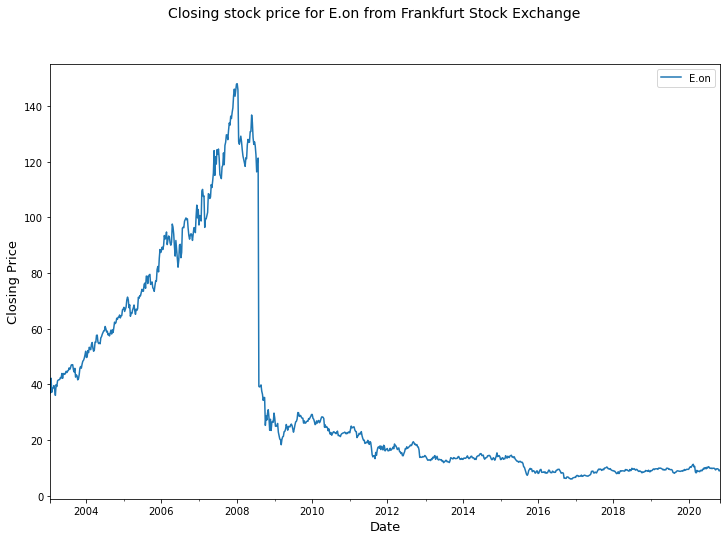
\includegraphics[scale=0.35]{images/Stock_Eon.png}
\end{center}
\end{frame}

%------------------------------------------------
\subsection{Information}
\begin{frame}
	\frametitle{Some additional information}
	\begin{itemize}
		\item The data was fetching from quandl.
		\item We used an API. The code can be found in the folder Python Code \cite{p1}.
		
	\end{itemize}
\end{frame}


%------------------------------------------------
%------------------------------------------------
\section{Case Study}
%------------------------------------------------
\subsection{Question 1}
\begin{frame}
\frametitle{Announcement Days}
\begin{table}[H]
	\centering
	\begin{tabular}{|l|l|l|}
		\toprule
		Acquirer & Target & Announcement Date \\\toprule
		AOT& Time Warner & January 10\textsuperscript{th}, 2000 \\
		AT\&T& Bellsouth& March 6\textsuperscript{th}, 2006\\
		Worldcom& MCI& November 10\textsuperscript{th}, 1997\\ \hline
	\end{tabular}
	\caption{Announcement days}
	\label{aanounce}
\end{table}
\end{frame}

%------------------------------------------------
\subsection{Question 2}
\begin{frame}
\frametitle{CAR's}
\begin{figure}[H]
	\centering
	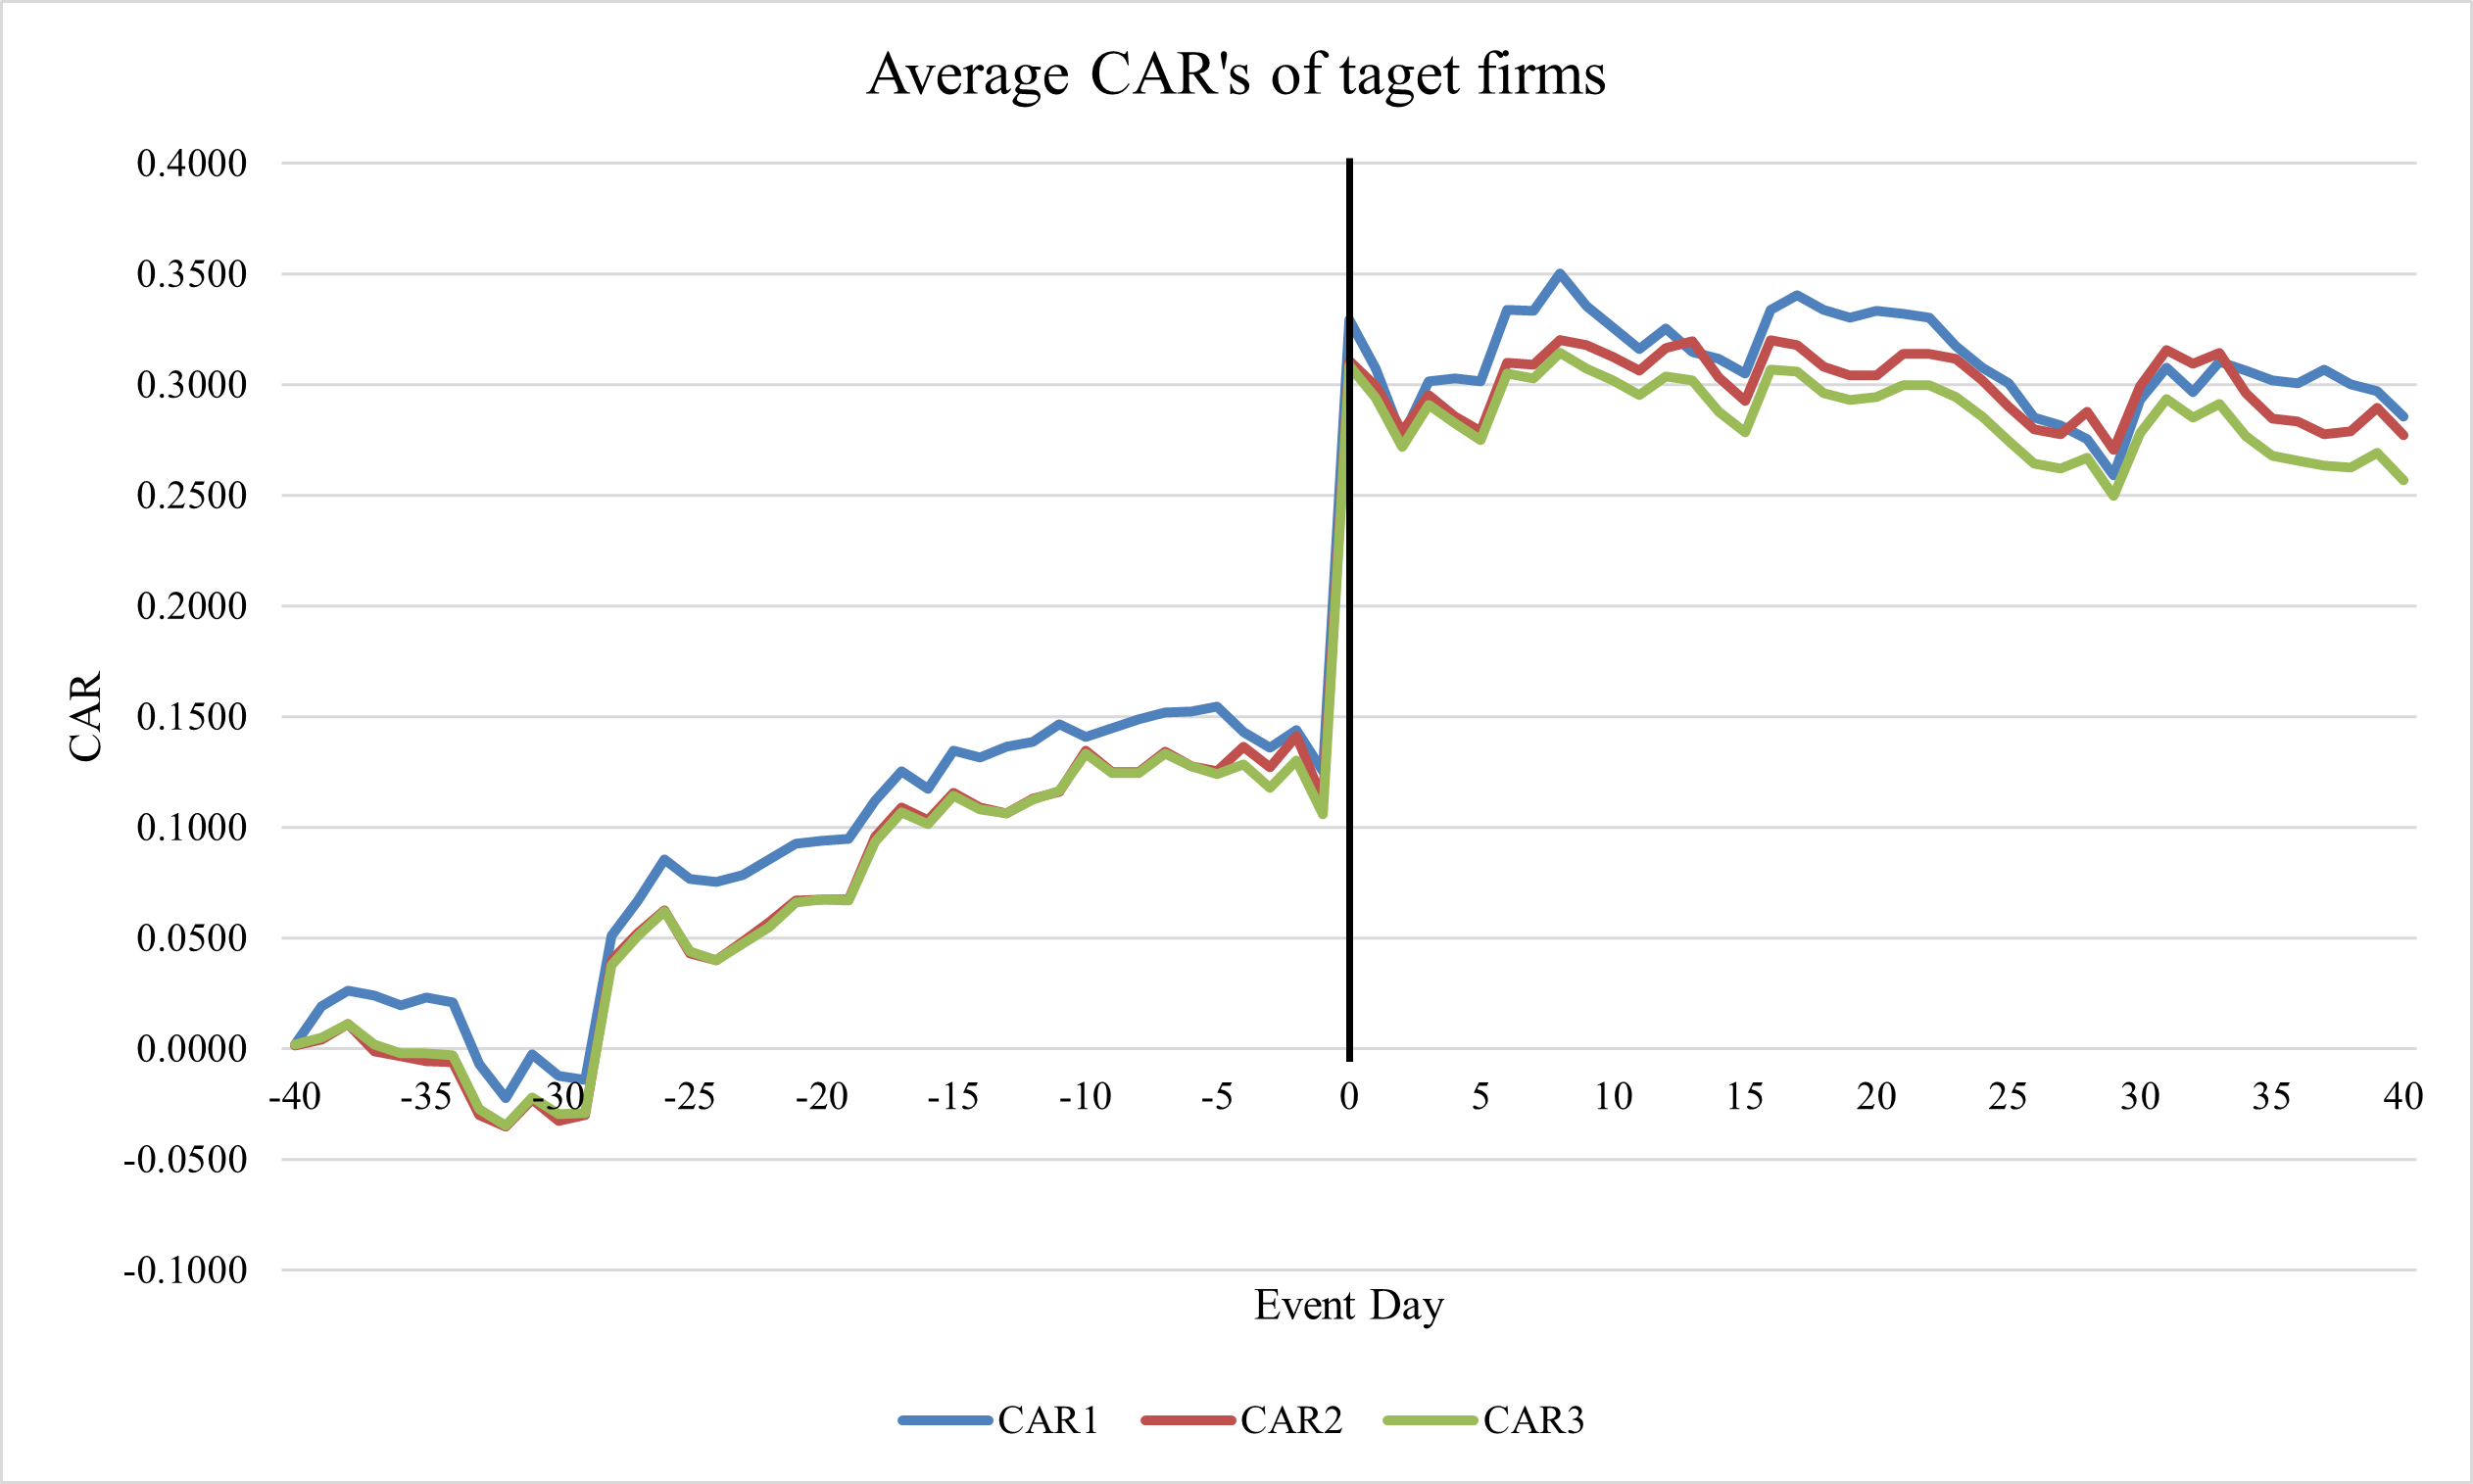
\includegraphics[scale=0.35]{images/Bild1.png}
	\caption{Target firms}
	\label{bildlitargets}
\end{figure}
\end{frame}

%------------------------------------------------

\begin{frame} % Need to use the fragile option when verbatim is used in the slide
\frametitle{Information Leak}
\begin{example}[Time Wartner]
	The previous graph suggests that no information leaked at the time Warner Transaction.
\end{example}
\begin{example}[Bellsouth]
	The previous graph suggests that some information leaked before the merger.
\end{example}
\end{frame}

%------------------------------------------------


\begin{frame}
	\frametitle{Information Leak}
	\begin{block}{Time Warner}
	The graph in figure \ref{bildlitargets} suggests that no information leaked on the TimeWarner transaction. In fact, prior to the announcement date CARs of the company were stable. \cite{p1}
	\end{block}
	
	\begin{block}{Bellsouth}
		Bellsouth and MCI, instead
		show that some information has been leaking prior to the announcement date, in particular if
		we look the MCI line.\cite{p1}
	\end{block}
	
	\begin{block}{MCI}
		 Curabitur condimentum, enim sed venenatis rutrum, ipsum neque consectetur orci, sed blandit justo nisi ac lacus. \cite{p1}
	\end{block}
\end{frame}

%------------------------------------------------
\subsection{Question 3}
\begin{frame}
	\frametitle{Significance of the results}
	\begin{columns}[c] % The "c" option specifies centered vertical alignment while the "t" option is used for top vertical alignment
		
		\column{.55\textwidth} % Left column and width
		\textbf{Concept}
		\begin{enumerate}
			\item Compute the t-stat.
			\item Compare with significance level.
			\item Judge if the variable being different tha n 0 is statistically significant.\cite{p1}
		\end{enumerate}
		
		\column{.4\textwidth} % Right column and width
		Lorem ipsum dolor sit amet, consectetur adipiscing elit. Sed volutpat ante purus, quis accumsan dolor.
		
	\end{columns}
\end{frame}

%------------------------------------------------

\begin{frame}
\frametitle{Abnormal Returns }
\begin{figure}[H]
	\centering
	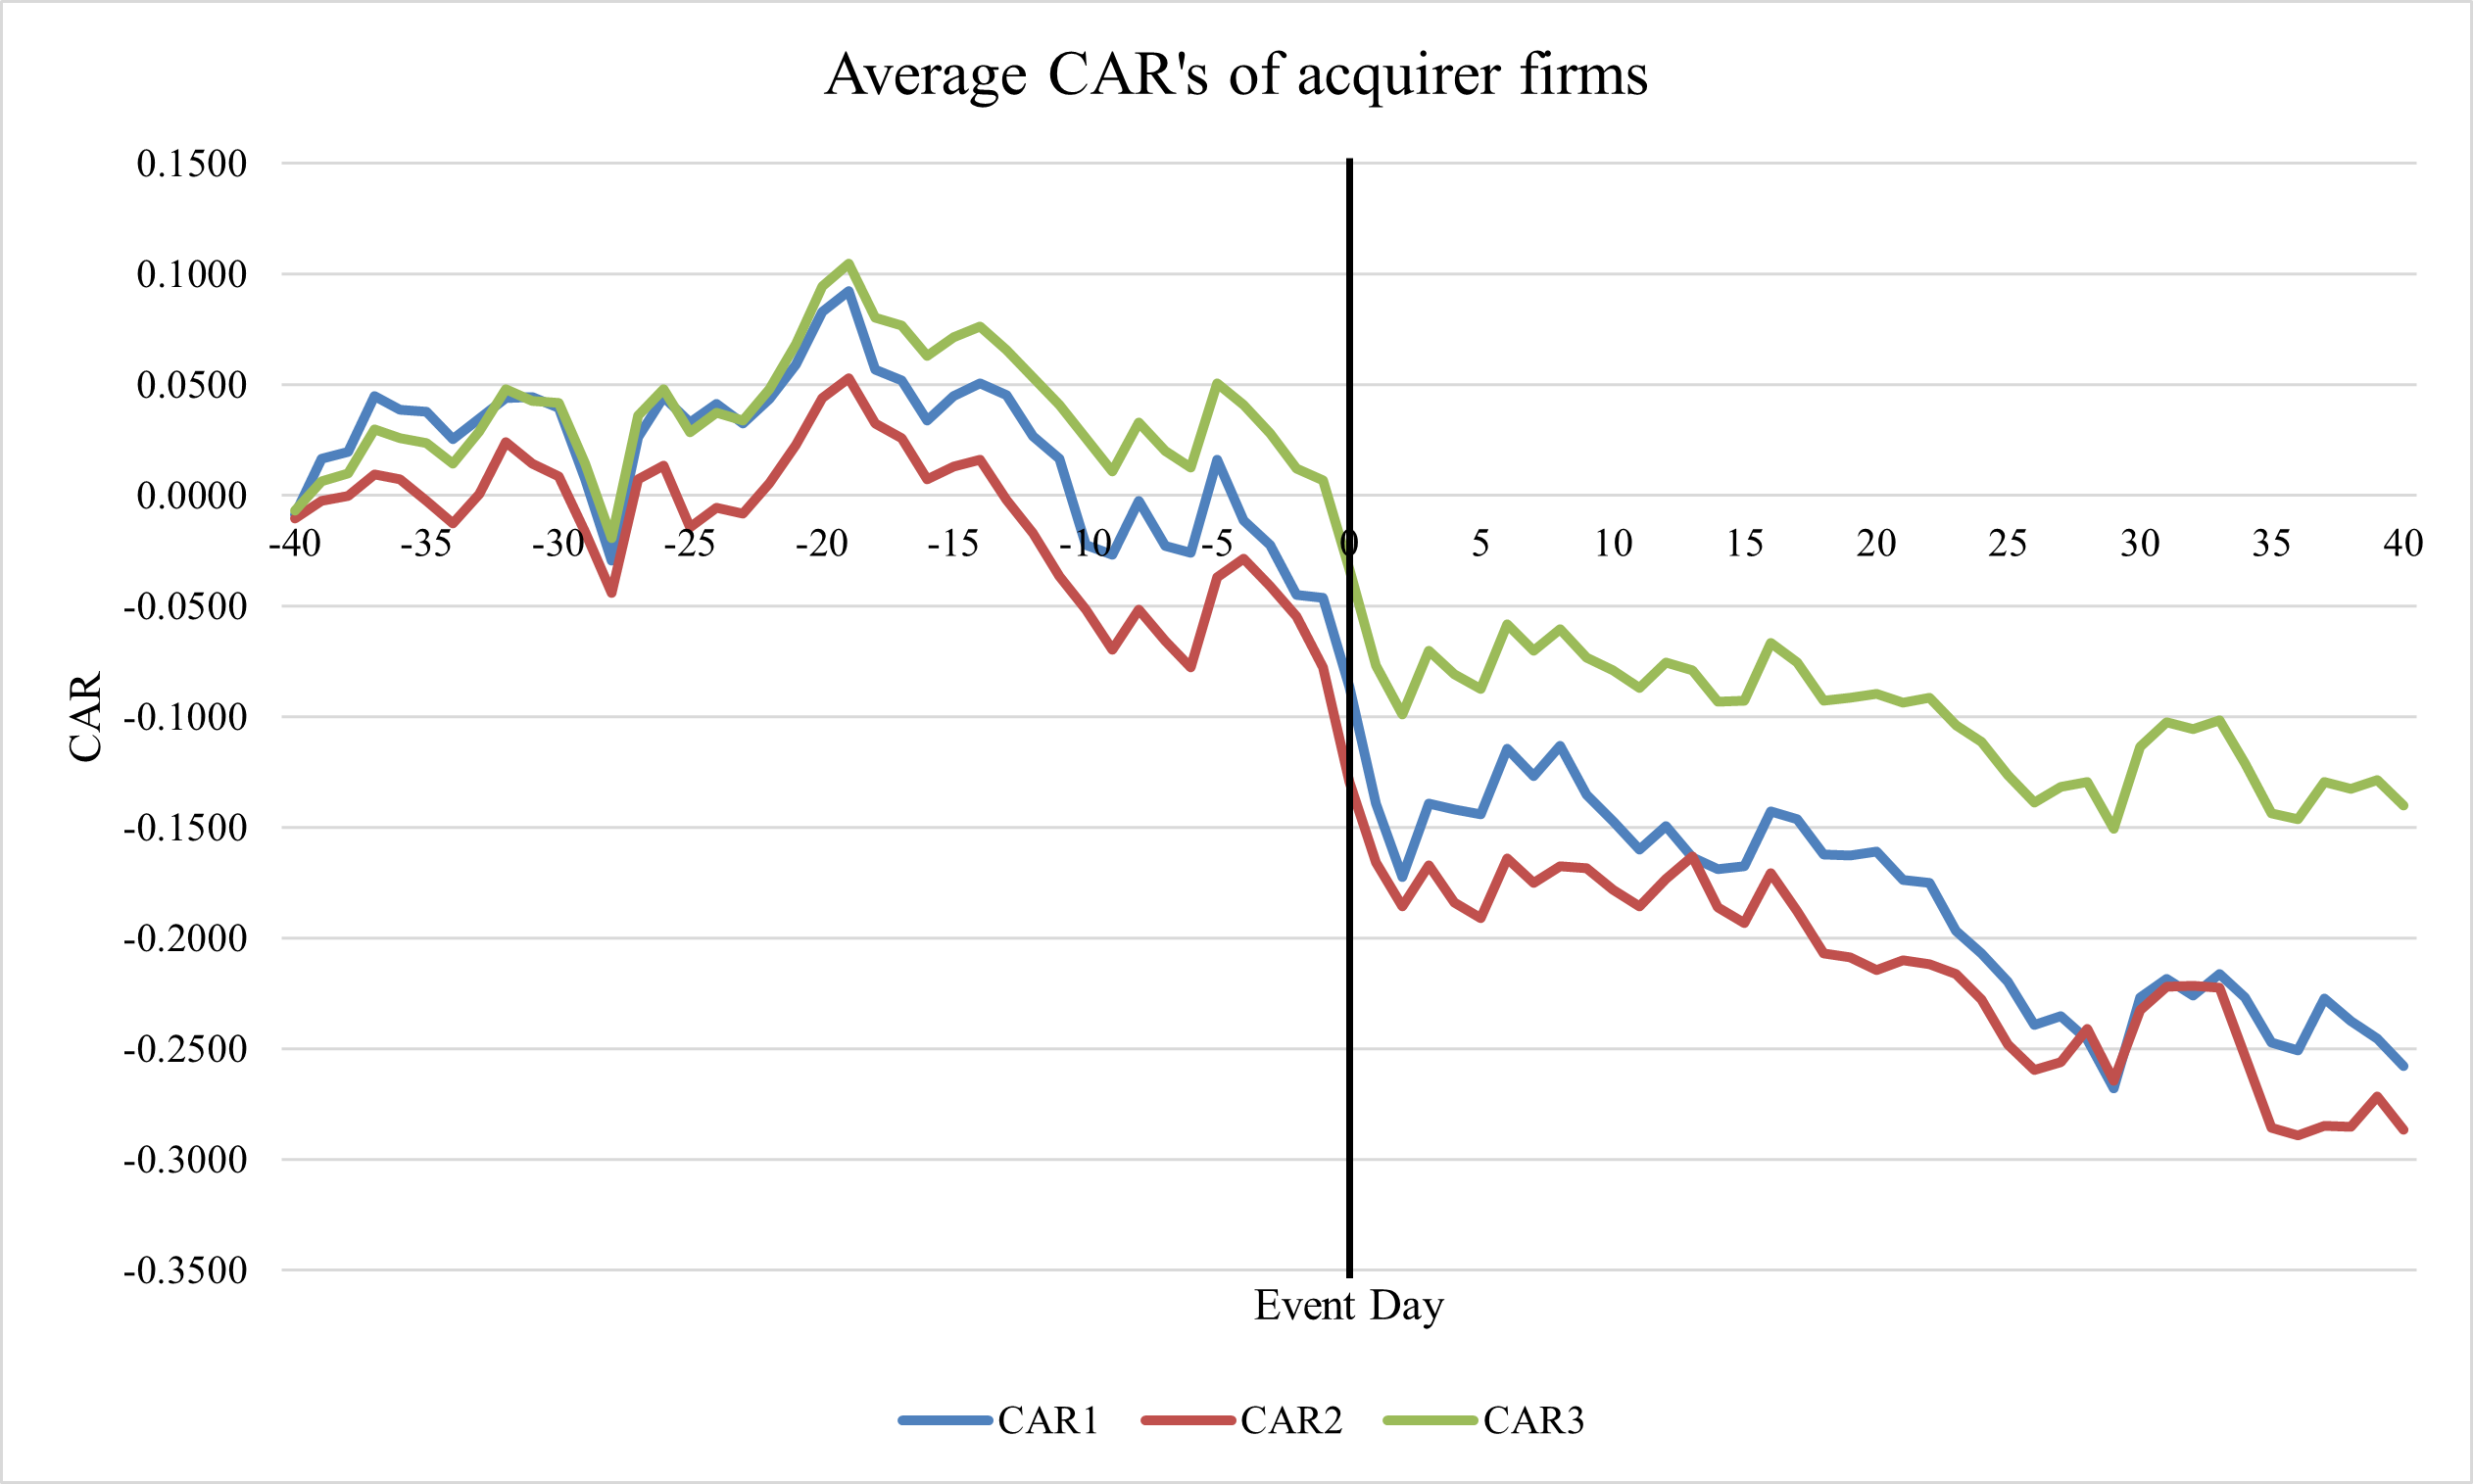
\includegraphics[scale=0.4]{images/Bild2.png}
	\caption{Acquirer firms}
	\label{bildlyacqui}
\end{figure}
\end{frame}

%------------------------------------------------
\section{References}
\subsection{References}
\begin{frame}
\frametitle{References}
\footnotesize{
\begin{thebibliography}{99} % Beamer does not support BibTeX so references must be inserted manually as below
\bibitem[Smith, 2012]{p1} John Smith (2012)
\newblock Title of the publication
\newblock \emph{Journal Name} 12(3), 45 -- 678.
\end{thebibliography}
}
\end{frame}

%------------------------------------------------
\section{Questions}
\subsection{Questions}
\begin{frame}
	\begin{center}
		\Large{
			Thank you for the attention! \\
			Questions are welcome.}
	\end{center}

\end{frame}

%----------------------------------------------------------------------------------------

\end{document} 